\documentclass[12pt,letterpaper]{article}
\usepackage{fullpage}
\usepackage[top=2cm, bottom=4.5cm, left=2.5cm, right=2.5cm]{geometry}
\usepackage{amsmath,amsthm,amsfonts,amssymb,amscd}
\usepackage{lastpage}
\usepackage{enumerate}
\usepackage{fancyhdr}
\usepackage{mathrsfs}
\usepackage{xcolor}
\usepackage{graphicx}
\usepackage{listings}
\usepackage{hyperref}
\usepackage{tikz}
\usepackage{xfrac}
\usepackage{nicefrac}
\usepackage{xcolor}

\usetikzlibrary{shapes.geometric,fit}

\hypersetup{
    colorlinks=true,
    linkcolor=blue,
    linkbordercolor={0 0 1}
}

\setlength{\parindent}{0.0in}
\setlength{\parskip}{0.05in}

\newcommand\course{ECON 3211}
\newcommand\hwnumber{3}
\newcommand\NetIDa{dc3451}
\newcommand\NetIDb{David Chen}          

\theoremstyle{definition}
\newtheorem*{statement}{Statement}
\newtheorem*{claim}{Claim}
\newtheorem*{theorem}{Theorem}

\newcommand{\contra}{\Rightarrow\!\Leftarrow}
\newcommand{\Lag}{\mathcal{L}}

\pagestyle{fancyplain}
\headheight 35pt
\lhead{\NetIDa}
\lhead{\NetIDa\\\NetIDb}
\chead{\textbf{\Large Problem Set \hwnumber}}
\rhead{\course \\ \today}
\lfoot{}
\cfoot{}
\rfoot{\small\thepage}
\headsep 1.5em

\begin{document}

\subsection*{Problem 1}
\subsection*{a), d)}

\begin{center}
    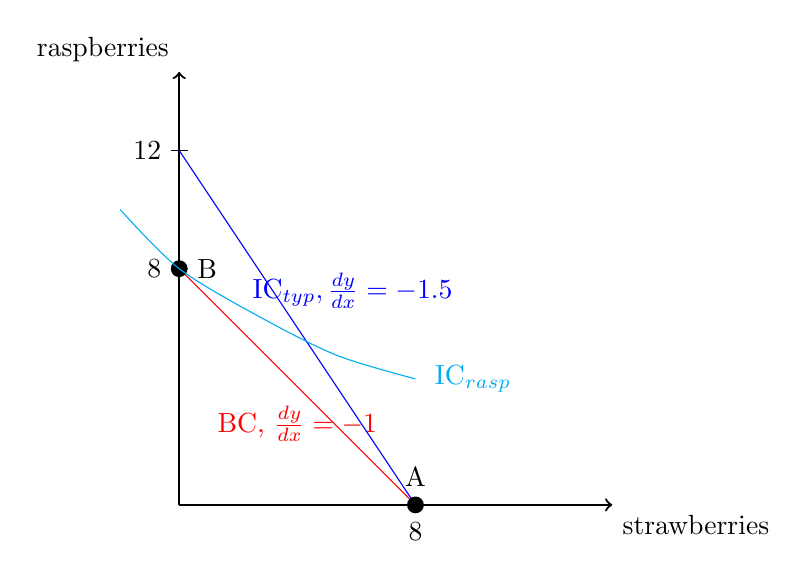
\begin{tikzpicture}[
            dot/.style={shape=circle, inner sep=2pt, draw, node contents=},
            circ/.style={shape=circle, inner sep=2pt, draw, fill}]
        \draw[thick,->] (0,0) -- (5.5,0) node[anchor=north west] {strawberries};
        \draw[thick,->] (0,0) -- (0,5.5) node[anchor=south east] {raspberries};
    
        \draw (3cm,3pt) -- (3cm,-3pt) node[anchor=north] {$8$}; 

        \draw (3pt,3cm) -- (-3pt,3cm) node[anchor=east] {$8$};
        \draw (3pt,4.5cm) -- (-3pt,4.5cm) node[anchor=east] {$12$};

        \draw[color=red] (0,3) -- node[label=below:{BC, $\frac{dy}{dx} = -1$}]{} (3,0);
        \draw[color=blue] (3,0) -- node[label=above:{IC$_{typ}, \frac{dy}{dx} = -1.5$},xshift=7mm]{} (0,4.5);
        \draw (3,0) node[circ,label=above:{A}]{};
        \draw (0,3) node[circ,label=right:{B}]{};

        \draw[color=cyan] plot[smooth] coordinates {(-0.75, 3.75) (0,3) (1, 2.4) (2, 1.9) (3,1.6)} node[label=right:{IC$_{rasp}$}]{};
        %\draw[thick] (2.5,4) -- (2.5,0.67) -- (4,0.67);
        %\draw (4,.67) node[label=right:IC]{};
        %\draw (2.5,0.67) node[circ,label=above right:{B$^*$, (5,500)}]{};
        
        %\draw[dashed] (2.5,0) -- (2.5,0.67);
        %\draw[dashed] (0,0.67) -- (2.5,0.67);
        %\draw[dashed] (0,0) -- (4,1.066);
    \end{tikzpicture}
\end{center}

\subsection*{b)}

\begin{align*}
    MU_X &= \frac{\delta U}{\delta x} = 3 \\
    MU_Y &= \frac{\delta U}{\delta y} = 2 \\
    MRS_{Y,X} &= -\frac{MU_X}{MU_Y} \\
    &= -\frac{3}{2} \\
\end{align*}

What this means is that, as $MRS_{Y,X}$ is invariant in respect to both $x, y$, then for varying amounts of strawberries and raspberries $MRS_{Y,X}$ is constant at $1.5$ for typical consumers.

\subsection*{c)}

As above, the marginal utilities for raspberries and strawberries are respectively 
$MU_Y=2$ and $MU_X = 3$. 
Now given that the prices of those two fruits are equal, 
then we have that an utility maximizing consumer buys only strawberries 
and no raspberries. This can be seen as $|MRS_{Y,X}| = 1.5 > \frac{p_X}{p_Y} = 1$.

\subsection*{d)}

The optimal bundle is labeled A.

\subsection*{e)}

To convince the typical consumer to purchase both, he ought to price raspberries 
such that $|MRS_{Y,X}| = \frac{p_x}{p_y} \implies 1.5 = \frac{3}{p_y} \implies p_y=\$2$ per pack.

\subsection*{f)}
\subsubsection*{f.1}
\begin{align*}
    \Lag (x, y, \lambda) &= x + 9ln(y) - \lambda(3x + 3y -24)
\end{align*}

\subsubsection*{f.2}
\begin{align*}
    \frac{\delta \Lag}{\delta x} &= 1 - 3\lambda\\
    \frac{\delta \Lag}{\delta y} &= \frac{9}{y} - 3\lambda \\
    \frac{\delta \Lag}{\delta \lambda} &= -3x - 3y + 24\\
\end{align*}

\subsubsection*{f.3}

\begin{alignat*}{2}
    && \frac{\delta \Lag}{\delta x} &= 1 - 3\lambda = 0 \\
    &\implies& \lambda &= \frac{1}{3} \\
    &\implies& \frac{\delta \Lag}{\delta y} &= \frac{9}{y} - 1 = 0 \\
    &\implies& y &= 9 \\
    &\implies& \frac{\delta \Lag}{\delta x} &= -3x -27 +24 = 0\\
    &\implies& x &= -1
\end{alignat*}

In this case, we cannot purchase a negative amount of strawberries, and thus have a
corner solution where only raspberries are bought.

\subsubsection*{f.4}

No, the raspberry lover (fittingly) only buys raspberries at the grocer's,
ignoring strawberries.

\subsection*{g)}

Note that the budget constraint is the same between the typical consumer and
the raspberry lover, as the grocer's prices and their budgets do not change.

Further, at the optimal bundle, labeled B, we have that $|MRS_{Y,X}| < \frac{p_x}{p_y}$.

\subsection*{h)}

If the grocer sells strawberries at $\$3$, then they need to sell raspberries at a
price such that when solving $-3x - 9p_y + 24 = 0$ we have a positive solution for $x$.
This means that he must charge less than $24/9 = \$2.66$ for the raspberries to
convince the raspberry lover to buy strawberries.

\subsection*{Problem 2}

\begin{center}
    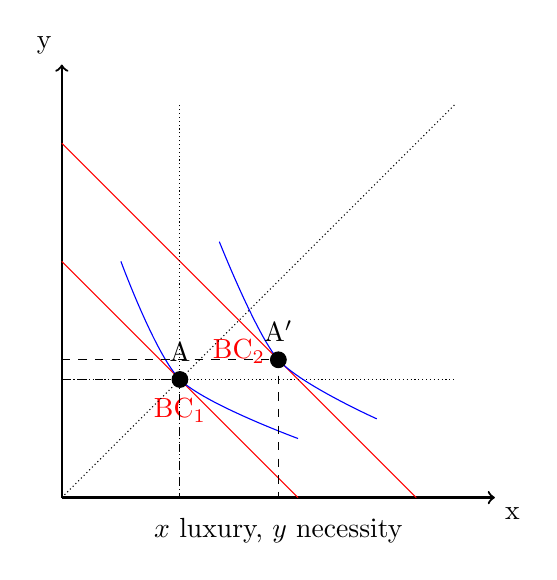
\begin{tikzpicture}[
            dot/.style={shape=circle, inner sep=2pt, draw, node contents=},
            circ/.style={shape=circle, inner sep=2pt, draw, fill}]
        \draw[thick,->] (0,0) -- node[label=below:{$x$ luxury, $y$ necessity}]{} (5.5,0) node[anchor=north west] {x};
        \draw[thick,->] (0,0) -- (0,5.5) node[anchor=south east] {y};
    

        \draw[color=red] (0,3) -- node[label=below:{BC$_1$}]{} (3,0);
        \draw[color=red] (0,4.5) -- node[label=below:{BC$_2$}]{} (4.5,0);

        \draw[color=blue] plot[smooth] coordinates {(0.75,3) (1.5,1.5) (3,0.75)};
        \draw[densely dotted] (0,0) -- (5,5);
        \draw[densely dotted] (0,1.5) -- (5,1.5);
        \draw[densely dotted] (1.5,0) -- (1.5,5);

        \draw[color=blue] plot[smooth] coordinates {(2,3.25) (2.75,1.75) (4,1)};

        \draw (1.5,1.5) node[circ,label=above:{A}]{};
        \draw (2.75,1.75) node[circ,label=above:{A$'$}]{};
        \draw[dashed] (0,1.75) -- (2.75,1.75) -- (2.75,0);
        \draw[dashed] (0,1.5) -- (1.5,1.5) -- (1.5,0);
    \end{tikzpicture}
\end{center}

\begin{center}
    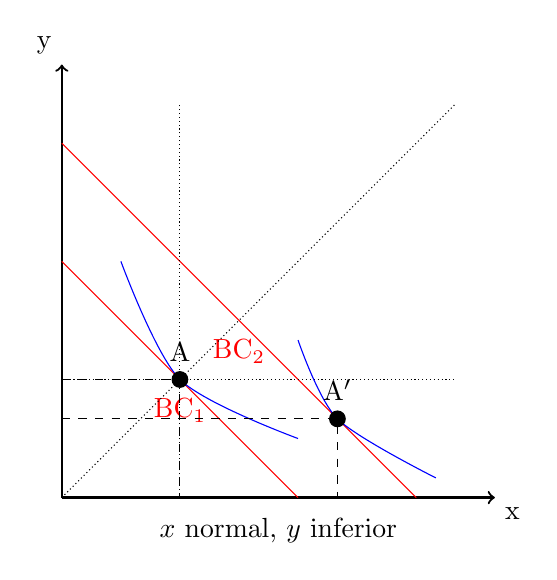
\begin{tikzpicture}[
            dot/.style={shape=circle, inner sep=2pt, draw, node contents=},
            circ/.style={shape=circle, inner sep=2pt, draw, fill}]
        \draw[thick,->] (0,0) -- node[label=below:{$x$ normal, $y$ inferior}]{} (5.5,0) node[anchor=north west] {x};
        \draw[thick,->] (0,0) -- (0,5.5) node[anchor=south east] {y};
    

        \draw[color=red] (0,3) -- node[label=below:{BC$_1$}]{} (3,0);
        \draw[color=red] (0,4.5) -- node[label=below:{BC$_2$}]{} (4.5,0);

        \draw[color=blue] plot[smooth] coordinates {(0.75,3) (1.5,1.5) (3,0.75)};
        \draw[densely dotted] (0,0) -- (5,5);
        \draw[densely dotted] (0,1.5) -- (5,1.5);
        \draw[densely dotted] (1.5,0) -- (1.5,5);

        \draw[color=blue] plot[smooth] coordinates {(3,2) (3.5,1) (4.75,0.25)};

        \draw (1.5,1.5) node[circ,label=above:{A}]{};
        \draw (3.5,1) node[circ,label=above:{A$'$}]{};

        \draw[dashed] (0,1) -- (3.5,1) -- (3.5,0);
        \draw[dashed] (0,1.5) -- (1.5,1.5) -- (1.5,0);
    \end{tikzpicture}
\end{center}

\begin{center}
    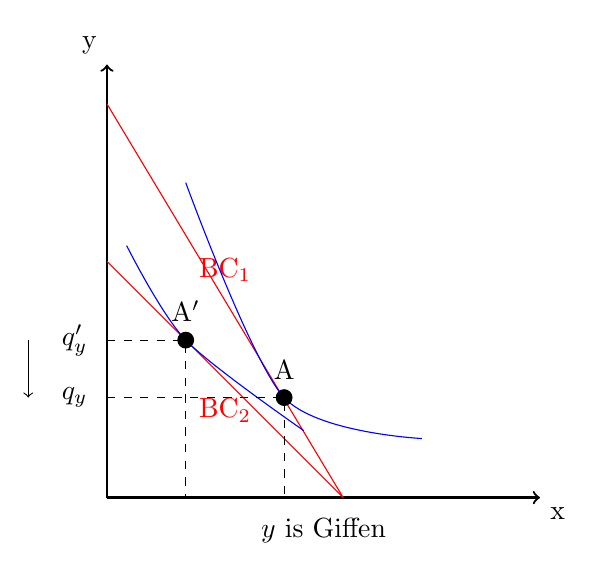
\begin{tikzpicture}[
            dot/.style={shape=circle, inner sep=2pt, draw, node contents=},
            circ/.style={shape=circle, inner sep=2pt, draw, fill}]
        \draw[thick,->] (0,0) -- node[label=below:{$y$ is Giffen}]{} (5.5,0) node[anchor=north west] {x};
        \draw[thick,->] (0,0) -- (0,5.5) node[anchor=south east] {y};
    

        \draw[color=red] (0,3) -- node[label=below:{BC$_2$}]{} (3,0);
        \draw[color=red] (0,5) -- node[label=above:{BC$_1$}]{} (3,0);

        \draw[color=blue] plot[smooth] coordinates {(0.25,3.2) (1,2) (2.5,0.85)};
        \draw[color=blue] plot[smooth] coordinates {(1,4) (2.25,1.27) (4,0.75)};

        \draw (1,2) node[circ,label=above:{A$'$}]{};
        \draw (2.25,1.27) node[circ,label=above:{A}]{};

        \draw[dashed] (0,2) node[label=left:{$q_y'$}]{} -- (1,2) -- (1,0);
        \draw[dashed] (0,1.27) node[label=left:{$q_y$}]{} -- (2.25,1.27) -- (2.25,0);

        \draw[->] (-1, 2) -- (-1,1.27);
    \end{tikzpicture}
\end{center}

\subsection*{Problem 3}

\subsubsection*{a)}
For a general Cobb-Douglass utility function $U(x,y) = x^\alpha y^{1-\alpha}$, we have 
that the Lagrangian method of optimization yields

\begin{alignat*}{2}
    &&\Lag (x,y,\lambda) &=  x^\alpha y^{1-\alpha} - \lambda (px_x + p_yy  - M)\\
    &&\frac{\delta \Lag}{\delta x} &= \alpha x^{\alpha - 1} y^{1-\alpha} -\lambda p_x = 0\\
    &&\frac{\delta \Lag}{\delta y} &= (1-\alpha)x^{\alpha}y^{-\alpha} - \lambda p_y=0\\
    &\implies& \frac{\alpha}{1 - \alpha} x^{-1}y &= \frac{p_x}{p_y} \\ 
    &\implies& y &= \frac{p_x}{p_y}\frac{1-\alpha}{\alpha}x \\
    &&\frac{\delta \Lag}{\delta \lambda} &= -p_xx - p_yy + M = 0 \\
    &\implies& M &= p_xx + p_x\frac{1-\alpha}{\alpha}x \\
    &&&= \frac{p_xx}{\alpha}
\end{alignat*}

Thus Ann's Engel curve for good $x$ takes the form of a straight line with slope $3p_x$.
This depends only on the price of $x$, but not $y$.

\subsubsection*{b)}

For perfect substitutes which satisfy a utility function $U(x,y) = \min[\alpha x, \beta y]$,
we have that interior solutions will always lie on the kink of the function,
or where $\alpha x = \beta y \implies y = \frac{\alpha}{\beta}x$.

In the budget constraint, this solves to $M = p_xx + p_y\frac{\alpha}{\beta}x =
(p_x + \frac{\alpha}{\beta}p_y)x$, so Bob's Engel curve is also a line, but
with slope $p_x+p_y$ such that $M = (p_x +p_y)x$.

This means that his Engel curve for good $x$ depends on both prices for $x$ and $y$.


\subsection*{Problem 4}
\subsection*{a)}
\begin{align*}
    \max_{x,y}[a^2ln(x) + y], \text{ s.t. } p_xx + y = M
\end{align*}

\subsection*{b)}

\begin{alignat*}{2}
    &&\Lag (x,y,\lambda) &= z^2ln(x) + y - \lambda(p_xx + y - M) \\
    &&\frac{\delta \Lag}{\delta x} &= \frac{z^2}{x} - \lambda p_x = 0 \\
    &&\frac{\delta \Lag}{\delta y} &= 1 - \lambda  = 0 \\
    &&\frac{\delta \Lag}{\delta \lambda} &= -p_xx - y + M = 0 \\
    &\implies& \lambda &= 1\\
    &\implies& \frac{z^2}{x} - p_x &= 0 \\
    &\implies& x &= \frac{z^2}{p_x} \\
    &\implies& -z^2 - y + M &= 0 \\
    &\implies& y &= M - z^2 \\
\end{alignat*}

Critically, we have that the demand for $x$ is $\frac{z^2}{p_x}$.

\subsection*{c)}
We take that for the rest of the problem that the solution is interior, 
as a corner solution would have that $x = \frac{M}{p_x}, y = 0$ and would
render analysis of the following inapplicable. 
In particular, we would have that the amount of $x$ demanded increases with $M$,
unlike in the case of an interior solution.

In the interior case, $x$ is neither normal nor inferior, as $\frac{\delta x}{\delta M} = 0$.

This also means that $x$ is not Giffen, as $\frac{\delta x}{\delta p_x} = -\frac{z^2}{p_x^2} < 0$.

\subsection*{d)}

We now have that the demand for $x$ is $x = \frac{p_x^2}{p_x} = p_x$, meaning that
as $\frac{\delta x}{\delta p_x} = 1 > 0$, we have that consumption of handbags
rises with price.

\subsection*{e)}

Goods whose consumption rises with price are called Veblen goods, or status symbol goods.
Demand increases with price because the good becomes a more effective means of conveying status.
Handbags in this case are an example of a Veblen good, but not a Giffen good.

Note that here as $U$ varies with $z = p_x$, we have that demand and the 
effective preferences of consumers change with the price of a good.
However, in a Giffen good, we see that budget constraints change such that optimization changes,
resulting in the rise in consumption with the rise of price. The demand for such
a good is not altered, like it is in this case.

\subsection*{Problem 5}

\subsubsection*{a),b)}

\begin{center}
    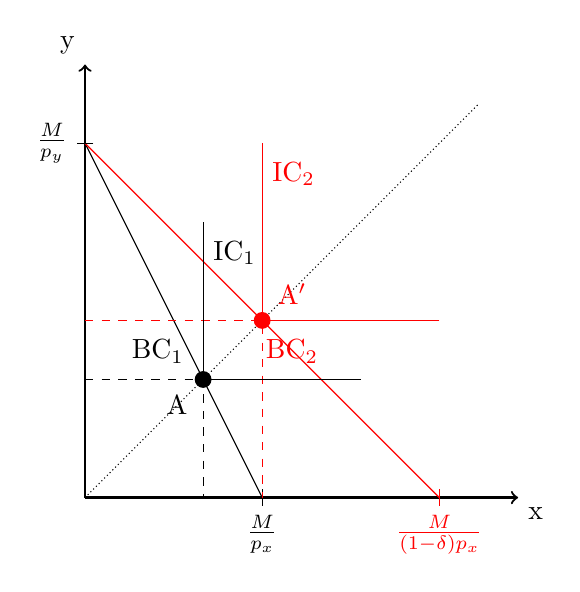
\begin{tikzpicture}[
            dot/.style={shape=circle, inner sep=2pt, draw, node contents=},
            circ/.style={shape=circle, inner sep=2pt, draw, fill}]
        \draw[thick,->] (0,0) -- (5.5,0) node[anchor=north west] {x};
        \draw[thick,->] (0,0) -- (0,5.5) node[anchor=south east] {y};

        \draw[color=black] (0,4.5) -- node[label=below:{BC$_1$},xshift=-2mm]{} (2.25,0);
        \draw[color=red] (0,4.5) -- node[label=below right:{BC$_2$},xshift=-2mm]{} (4.5,0);

        \draw[color=red] (4.5cm,3pt) -- (4.5cm,-3pt) node[anchor=north] {$\frac{M}{(1-\delta)p_x}$}; 
        \draw[color=black] (2.25cm,3pt) -- (2.25cm,-3pt) node[anchor=north] {$\frac{M}{p_x}$}; 

        \draw (3pt,4.5cm) -- (-3pt,4.5cm) node[anchor=east] {$\frac{M}{p_y}$};

        \draw[color=red,dashed] (0,2.25) -- (2.25,2.25) -- (2.25,0); 
        \draw[color=black,dashed] (0,1.5) -- (1.5,1.5) -- (1.5,0);


        \draw[densely dotted] (0,0) -- (5,5);

        \draw[color=red] (4.5,2.25) -- (2.25,2.25) -- (2.25,4.5) node[label=below:{IC$_2$},xshift=4mm]{}; 
        \draw[color=black] (3.5,1.5) -- (1.5,1.5) -- (1.5,3.5) node[label=below:{IC$_1$},xshift=4mm]{};

        \draw[color=red] (2.25,2.25) node[circ,label=above right:{A$'$}]{};
        \draw[color=black] (1.5,1.5) node[circ,label=below left:{A}]{};
    \end{tikzpicture}
\end{center}

\subsubsection*{c)}

\begin{center}
    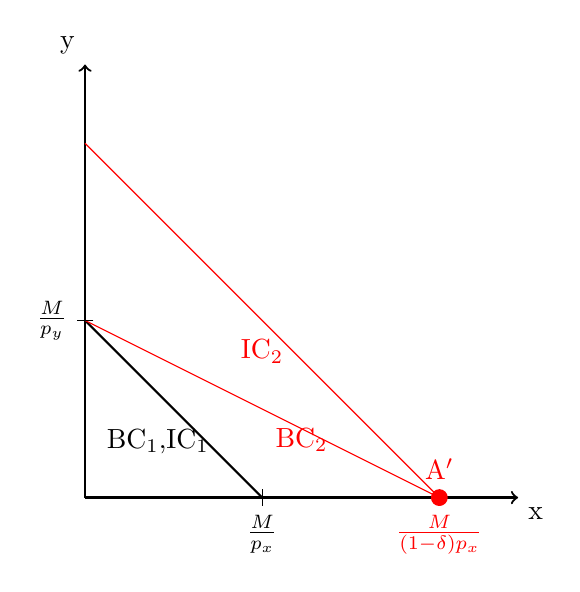
\begin{tikzpicture}[
            dot/.style={shape=circle, inner sep=2pt, draw, node contents=},
            circ/.style={shape=circle, inner sep=2pt, draw, fill}]
        \draw[thick,->] (0,0) -- (5.5,0) node[anchor=north west] {x};
        \draw[thick,->] (0,0) -- (0,5.5) node[anchor=south east] {y};

        \draw[thick,color=black] (0,2.25) -- node[label=below:{BC$_1$,IC$_1$},xshift=-2mm]{} (2.25,0);
        \draw[color=red] (0,2.25) -- node[label=below:{BC$_2$},xshift=5mm]{} (4.5,0);

        \draw[color=red] (0,4.5) --node[label=below:{IC$_2$}]{} (4.5,0); 

        \draw[color=red] (4.5cm,3pt) -- (4.5cm,-3pt) node[anchor=north] {$\frac{M}{(1-\delta)p_x}$}; 
        \draw[color=black] (2.25cm,3pt) -- (2.25cm,-3pt) node[anchor=north] {$\frac{M}{p_x}$}; 

        \draw (3pt,2.25cm) -- (-3pt,2.25cm) node[anchor=east] {$\frac{M}{p_y}$};

        \draw[color=red] (4.5,0) node[circ,label=above:{A$'$}]{};
    \end{tikzpicture}
\end{center}

Note that the optimal bundle can initially be anywhere on the budget constraint,
but after the price change the consumer only buys good $x$, moving the optimal bundle to A$'$.

\subsubsection*{d)}

In Problem 3, I show that for a Cobb-Douglass utility function of this form
utility is maximized when $q_y = \frac{p_x}{p_y}\frac{1-\alpha}{\alpha}q_x$ 
($q_x, q_y$ were previously denoted $x,y$ in Problem 3).

Substituting into the budget constraint,
we have that $p_xq_x + \frac{1-\alpha}{\alpha}p_xq_x = M
\implies q_x = \frac{\alpha M}{p_x}$

Similarly, we have that $q_x = \frac{p_y}{p_x}\frac{\alpha}{1-\alpha}q_y$.
Substituting into the budget constraint,
we have that $\frac{\alpha}{1-\alpha}p_yq_y + p_yq_y = M
\implies q_y = \frac{(1-\alpha)M}{p_y}$.

Now, accounting for a price change, we put $q_x = \frac{\alpha M}{(1-\delta)p_x}$.

Then, $\frac{dq_x}{d\delta} = \frac{\alpha M}{(1-\delta)^2p_x} > 0$,
so demand is increasing with a discount on $x$.

Further, note that $q_y$ is independent of $p_x$ ($\frac{dq_y}{d\delta} =0$), 
and so this is not affected by a discount
on $x$ in the Cobb-Douglass case.

\end{document}